\chapter{Motor de inferencia para Redes Neuronales Bayesianas} \label{ch:motor_inferencia}

\section{Biblioteca desarrollada en C}

Cómo las bibliotecas estándar no ofrecen soporte para la inferencia de BNN en plataformas de bajas prestaciones, en consecuencia, se ha desarrollado una biblioteca de funciones que ejecutan la inferencia de capas BNN estándar y convolucionales con funciones de activación ReLU o exponenciales normalizadas (SoftMax) utilizando precisión de coma fija. Esta biblioteca se ha desarrollado en C y se muestra en la Figura \ref{fig:experiment_pipeline} como el componente número 3. A continuación, se describe brevemente las principales decisiones de diseño.

\subsection{Aproximación de la función logaritmo}

Para calcular las métricas de incertidumbre se utiliza la función logaritmo por lo que se ha implementado una versión del algoritmo desarrollado por Turner para calcular el logaritmo de un número en coma fija \cite{binary_log}.

\subsection{Aproximación de la función SoftMax}

La función de activación SoftMax se utiliza en la última capa de una NN para transformar su vector de salida de forma que la suma de todos sus componentes sea 1, lo que facilita su interpretación. Mientras que calcular la función de activación ReLU es trivial, la función SoftMax no, por lo que una de las contribuciones de este trabajo ha sido crear una aproximación de esta función. La función SoftMax toma un vector de componentes $x \in X$ de tamaño $N$ como entrada y devuelve otro del mismo tamaño cuyos componentes $y\in Y$ se calculan según la Ecuación \ref{eq:softmax}.

\begin{equation} \label{eq:softmax}
y_i = \dfrac{e^{x_i}}{\sum_{j = 0}^N e^{x_j}}
\end{equation}

Para calcular esta función utilizando coma fija es necesario calcular la función exponencial en dicho formato. Para evitar desbordamientos de la función exponencial se va a utilizar la función SoftMax equivalente mostrada en la Ecuación \ref{eq:softmax_neg}.

\begin{equation} \label{eq:softmax_neg}
y_i = \dfrac{e^{x_i - \max(X)}}{\sum_{j = 0}^N e^{x_j - \max(X)}}
\end{equation}

Como se cumple que $x_i - \max(X) \in (-\infty, 0]$ entonces se cumple que $e^{x_i} \in (0,1]$. Para calcular la función exponencial en dicho rango se va a utilizar la Ecuación \ref{eq:split_exp}, dividiendo la entrada $x_i$ en su parte entera $a_i$ y su parte decimal $b_i$.
\begin{equation} \label{eq:split_exp}
e^{x_i} = e^{a_i+b_i} = e^{a_i} e^{b_i}
\end{equation}

La parte entera $e^{a_i}$ se calcula mediante una LUT de 20 entradas para el rango $[e^{-19}, e^{0}]$. A partir de $e^{-19}$ los valores son demasiado pequeños como para representarlos con la precisión disponible por lo que siempre toman el valor $0$. La parte decimal $e^{b_i}$ se aproxima mediante los 8 primeros términos de la serie de Taylor mostrada en la Ecuación \ref{eq:exp_taylor}. Para optimizar su cálculo evitando las instrucciones de división, los valores de $\dfrac{1}{n!}$ para $n \in [2,7]$ se han almacenado en una LUT.
\begin{equation} \label{eq:exp_taylor}
e^{b_i} \approx \sum_{n=0}^{7} \dfrac{{b_i}^n}{n!}
\end{equation}

La Figura \ref{fig:exp_aprox} muestra un estudio de la precisión de la aproximación. Se comparan sus resultados con los de la implementación de la función exponencial de la biblioteca estándar en punto flotante. Como medida cuantitativa del error se ha utilizado el error cuadrático medio (\textit{\textbf{M}ean \textbf{S}quared \textbf{E}rror}). Se aprecia cómo se obtiene un MSE muy bajo en el rango deseado, lo que implica que es una buena aproximación.

\begin{figure}[h]
	\centering
	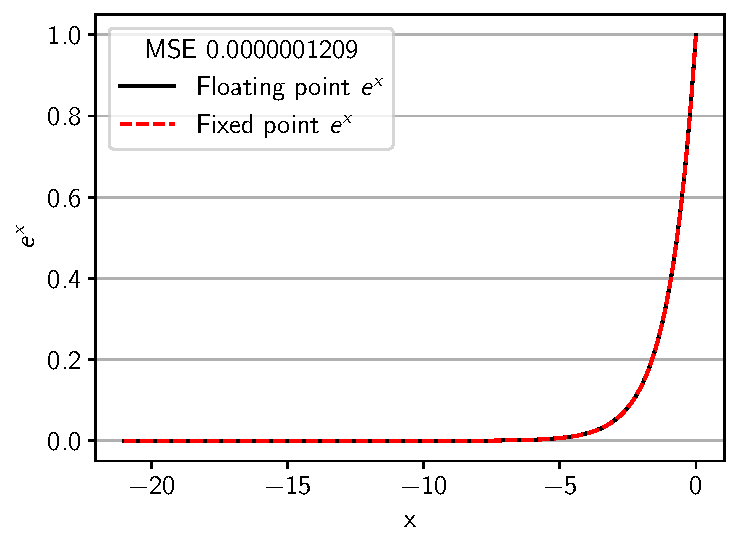
\includegraphics[width=0.55\linewidth]{root/Imagenes/bnn_lib/exp_aprox.pdf}
	\caption{Comparación de la función $e^x$ de la biblioteca estándar en punto flotante (línea negra) con la aproximación en coma fija implementada (línea roja discontinua) en el rango $[-20,0]$.}
	\label{fig:exp_aprox}
\end{figure}

\subsection{Muestreo de distribuciones Gaussianas}

Como se ha explicado previamente, las BNN necesitan muestrear distribuciones Gaussianas. Como método de muestreo base se ha utilizado un algoritmo basado en la suma de distribuciones uniformes, dicha suma se aproxima a una distribución gaussiana debido al TCL, como se muestra en la Ecuación \ref{eq:tcl_unif}.
\begin{equation} \label{eq:tcl_unif}
\sum_{n=0}^{N} \mathcal{U}_n(0,1) \sim \mathcal{N} \left( \dfrac{N}{2}, \sqrt{\dfrac{N}{12}} \right)
\end{equation}

El algoritmo implementado genera muestras de $\mathcal{N}(0,1)$ para luego transformarlas en muestras de una distribución gaussiana arbitraria $\mathcal{N}(\mu, \sigma)$ de media $\mu$ y desviación típica $\sigma$ utilizando la Ecuación \ref{eq:gauss_linear}.
\begin{equation} \label{eq:gauss_linear}
\mathcal{N}(\mu, \sigma) = \sigma \mathcal{N}(0,1) + \mu
\end{equation}

La aproximación empleada utiliza la suma de 12 distribuciones uniformes de forma que la desviación típica de la distribución resultante sea 1, lo que permite centrar la distribución como muestra la Ecuación \ref{eq:tcl_12center}.
\begin{equation} \label{eq:tcl_12center}
\sum_{n=0}^{12} \mathcal{U}_n(0,1) - 6 \sim \mathcal{N}(0,1)
\end{equation}

La Figura \ref{fig:gauss_aprox} muestra un análisis estadístico del método de muestreo implementado. En el gráfico Q-Q se aprecia cómo los cuantiles del conjunto de muestras son muy parecidos a los cuantiles teóricos, mostrando desviaciones en las colas cómo es de esperar de esta aproximación. En el histograma se aprecia cómo las muestras se ajustan bien a la distribución teórica.

\begin{figure}[h]
	\centering
	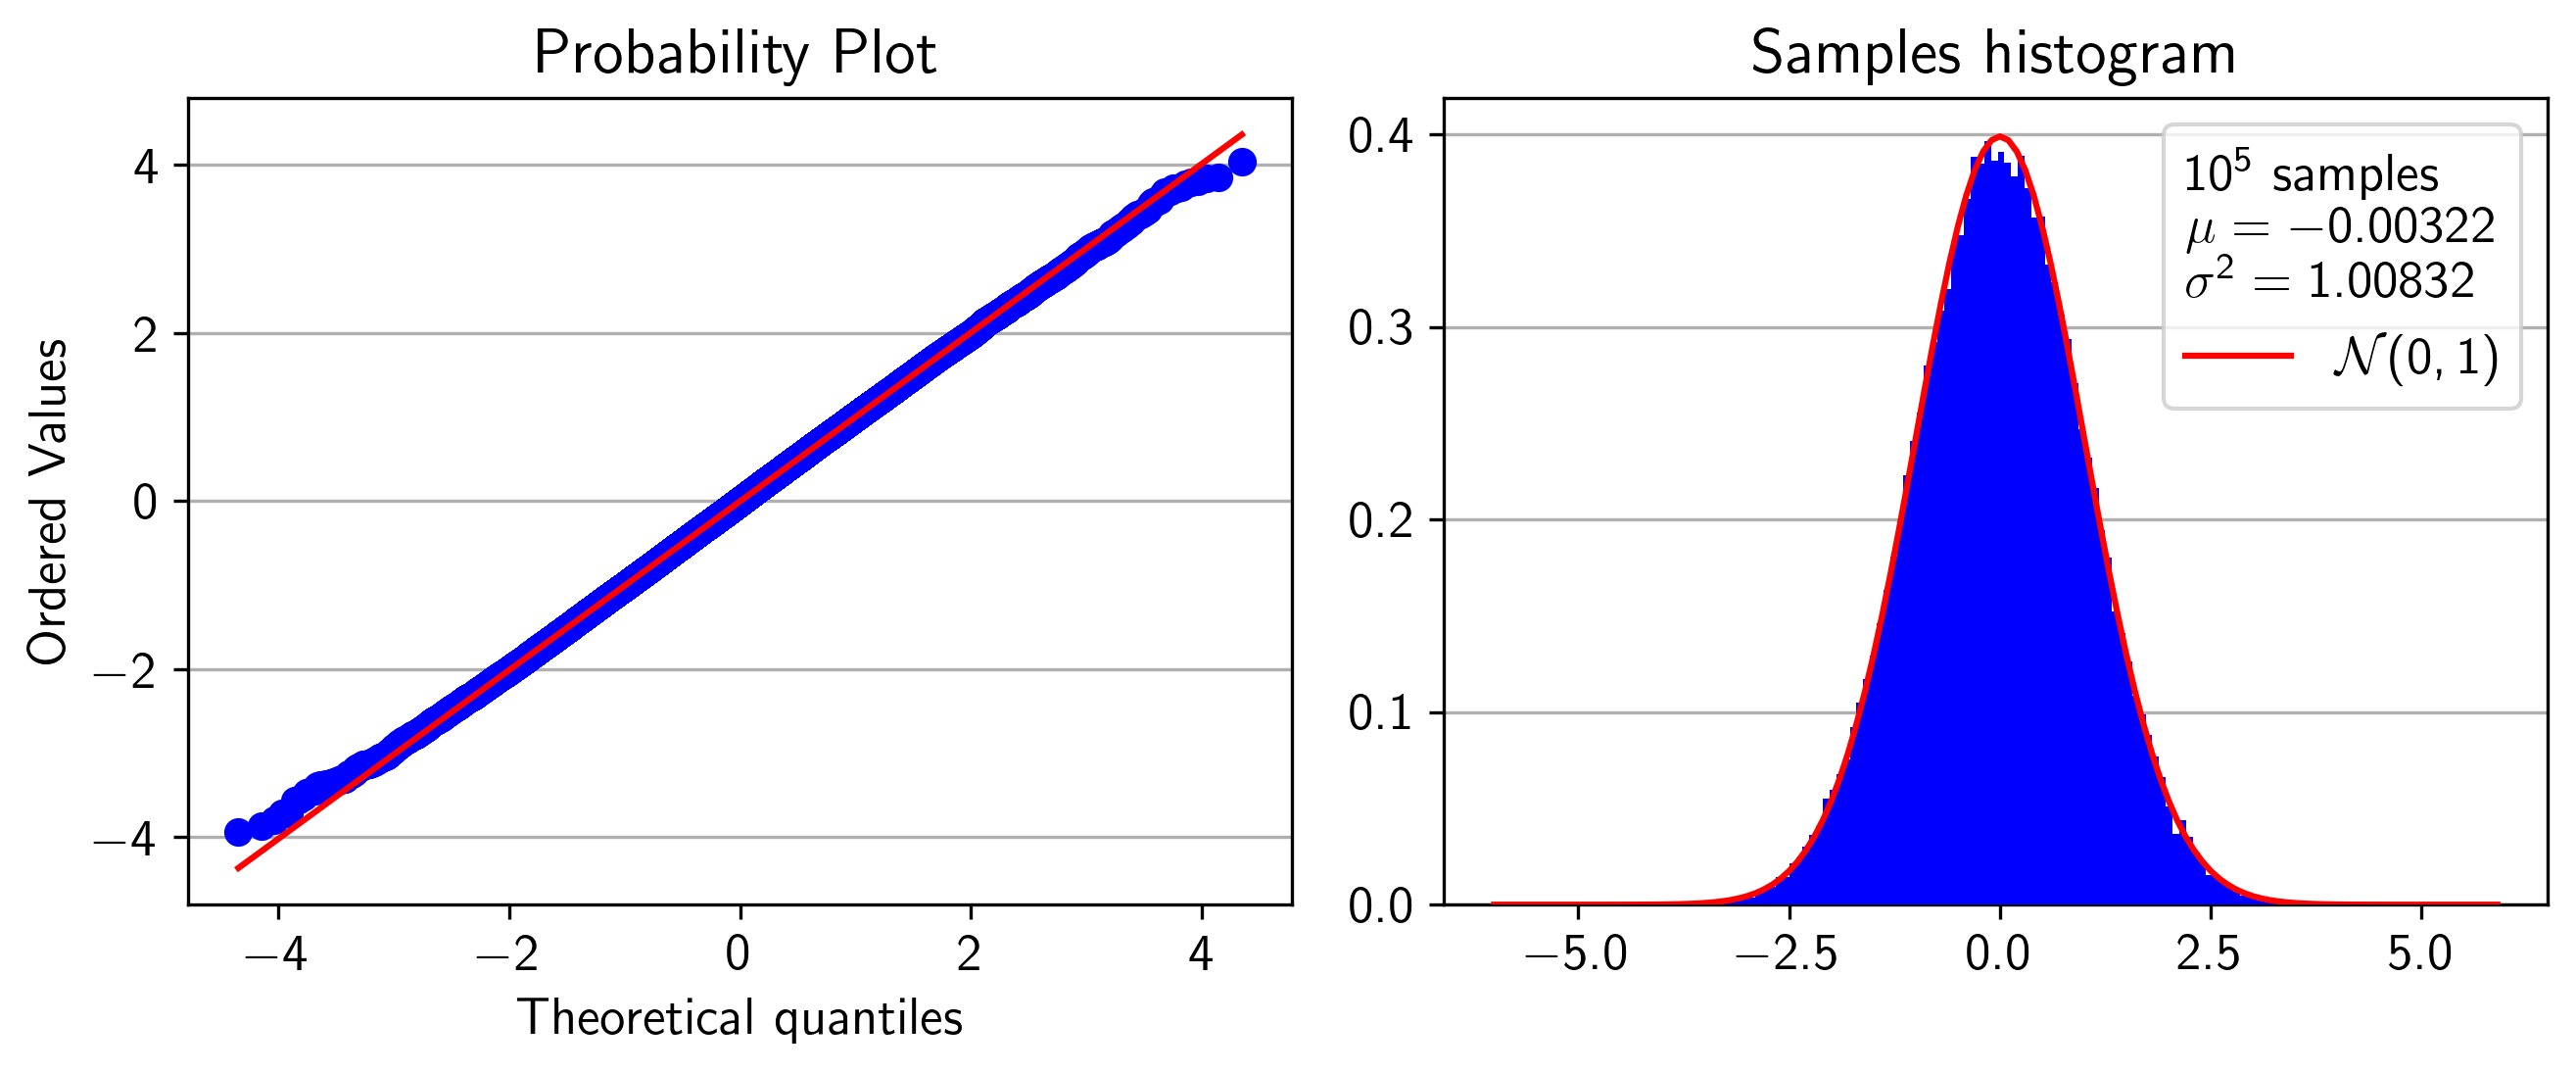
\includegraphics[width=\textwidth]{root/Imagenes/bnn_lib/gaus_aprox.png}
	\caption{Análisis estadístico de $10^5$ muestras del GRNG implementado (azul) con respecto a $\mathcal{N}(0,1)$ (rojo). A la izquierda se muestra un gráfico Q-Q. A la derecha se muestra un histograma.}
	\label{fig:gauss_aprox}
\end{figure}

\subsection{Muestreo de distribuciones Uniformes}

Generar muestras de distribuciones uniformes es una parte del algoritmo para generar muestras de una distribución gaussiana explicado previamente. Para hacerlo se utiliza una versión del algoritmo Xorshift de 32 bits \cite{xorshift}. Es un algoritmo sencillo y de bajo coste para generar números pseudoaleatorios uniformes solamente mediante instrucciones \texttt{xor} y \texttt{shift}.

\section{Análisis de resultados} \label{sec:uncertainty_example}

La Tabla \ref{tab:engine_acc} muestra la precisión obtenida con los diferentes modelos utilizando ambos motores de inferencia. Al tratarse de modelos probabilísticos pequeñas fluctuaciones son esperables, especialmente en las predicciones con mucha incertidumbre.

\begin{table}[h]
\centering
\caption{Comparación de precisión obtenida con el motor de inferencia implementado con respecto a resultados obtenidos con TensorFlow}
\label{tab:engine_acc}
\begin{tabular}{lll}
\hline
 &  \multicolumn{2}{c}{\textbf{Motor de inferencia}}\\
 \textbf{Modelo} & \textit{TensorFlow} & \textit{C} \\ \hline
 Hiperespectral BO   & 0.9039 & 0.9101 \\
 Hiperespectral IP   & 0.8139 & 0.8148 \\
 Hiperespectral KSC  & 0.9256 & 0.9217 \\
 Hiperespectral PU   & 0.9017 & 0.9021 \\
 Hiperespectral SV   & 0.9257 & 0.9275 \\
 Lenet-5 MNIST  	& 0.9836 & 0.9830 \\
 Lenet-5 CIFAR10	& 0.6351 & 0.6229 \\
 B2N2 MNIST     	& 0.9872 & 0.9854 \\
 B2N2 CIFAR10   	& 0.7295 & 0.7134 \\\hline
\end{tabular}
\end{table}

La Figura \ref{fig:figure_example} muestra un ejemplo de las gráficas utilizadas para validar las métricas de incertidumbre y propiedades estadísticas. Estas gráficas se han creado utilizando las predicciones para el conjunto de datos de píxeles hiperespectrales KSC.

La Subfigura~\ref{fig:example_hist} muestra un histograma de la incertidumbre agrupada por aciertos y fallos. La Subfigura~\ref{fig:example_class} muestra la incertidumbre media, separada en epistémica y aleatoria, de las predicciones de cada clase. La Subfigura~\ref{fig:example_acc_unc} muestra la precisión con respecto a la incertidumbre junto con un histograma de los datos agrupados también con respecto a la incertidumbre. Y finalmente, la Subfigura~ \ref{fig:example_calibration} muestra la recta de calibración del modelo.

Como se muestra en el ejemplo se obtienen resultados muy similares en todas las gráficas. Las únicas diferencias notables se aprecian en las rectas de precisión de la Figura \ref{fig:example_acc_unc}, pero estas diferencias ocurren en predicciones con incertidumbre alta de las que además hay muy pocas. El modelo al reportar una incertidumbre elevada ya está avisando de la baja fiabilidad de la predicción con lo que las diferencias en este tipo de predicciones son esperables y aceptables. Para el resto de modelos se obtienen resultados con las mismas similitudes entre motores de inferencia, se pueden consultar todos en el Anexo \ref{anx:motor}.

En conjunto, los resultados demuestran que el motor de inferencia desarrollado no perjudica ni las métricas de incertidumbre ni la precisión de los modelos incluso tras transformar los datos a coma fija perdiendo precisión en la representación.

% La pongo aqui para evitar errores de formato de las páginas
\begin{figure}[h]
 	\centering
 	\begin{subfigure}[b]{0.48\textwidth}
     	\centering
     	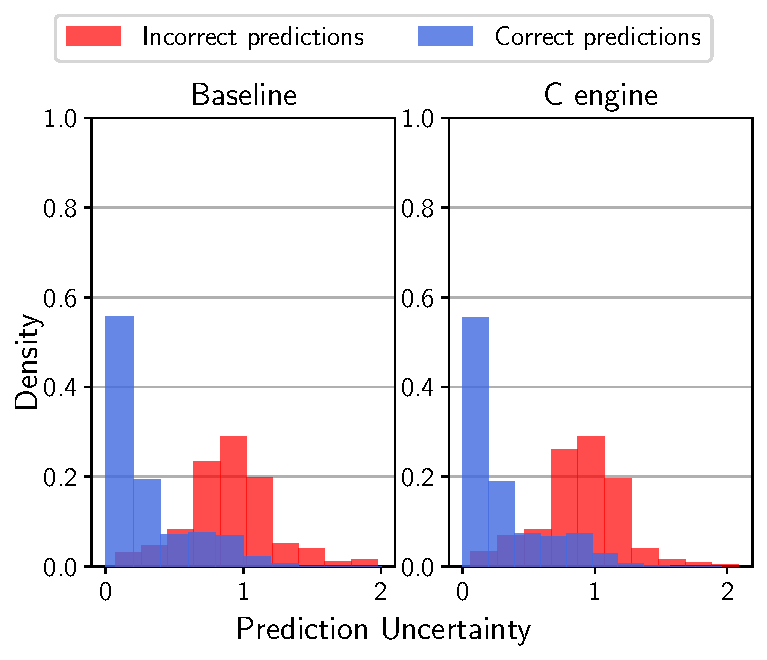
\includegraphics[width=\textwidth]{root/Imagenes/bnn_lib/hist_predictions.pdf}
     	\caption{Histogramas de incertidumbre divididos en predicciones incorrectas (rojo) y predicciones correctas (azul).}
     	\label{fig:example_hist}
 	\end{subfigure}
 	\hfill
 	\begin{subfigure}[b]{0.48\textwidth}
     	\centering
     	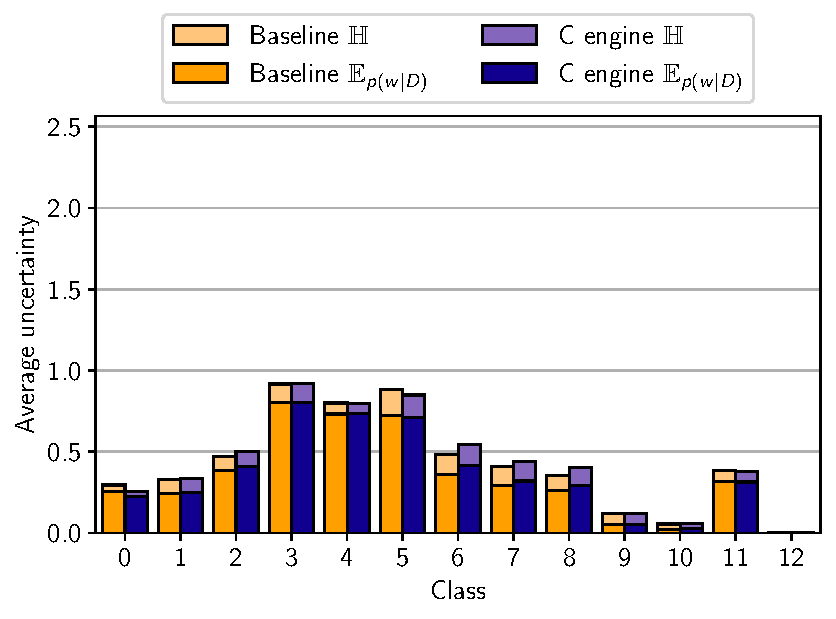
\includegraphics[width=\textwidth]{root/Imagenes/bnn_lib/class_uncertainty.pdf}
     	\caption{Incertidumbre predictiva ($\mathbb{H}$) y aleatoria ($\mathbb{E}p$) agrupada por clases.\\}
     	\label{fig:example_class}
 	\end{subfigure}
 	\hfill
 	\begin{subfigure}[b]{0.48\textwidth}
     	\centering
     	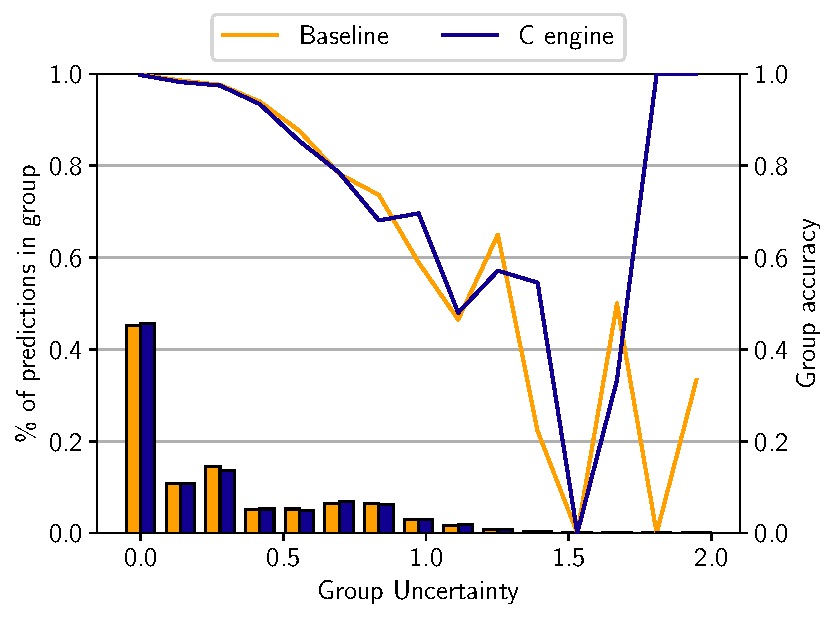
\includegraphics[width=\textwidth]{root/Imagenes/bnn_lib/acc_vs_unc.pdf}
     	\caption{Precisión (líneas) y porcentaje de predicciones (barras) agrupadas por incertidumbre.}
     	\label{fig:example_acc_unc}
 	\end{subfigure}
 	\hfill
 	\begin{subfigure}[b]{0.48\textwidth}
     	\centering
     	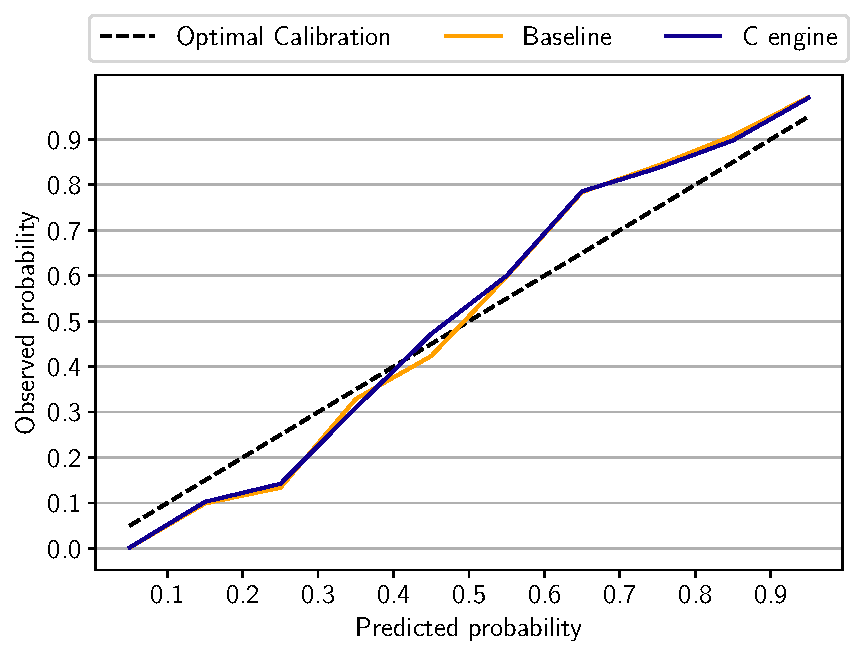
\includegraphics[width=\textwidth]{root/Imagenes/bnn_lib/calibration.pdf}
     	\caption{Recta de calibración del modelo, muestra probabilidades observadas con respecto a las probabilidades predichas por el modelo.}
     	\label{fig:example_calibration}
 	\end{subfigure}
    	\caption{Ejemplos de gráficas para analizar la incertidumbre y propiedades estadísticas de un modelo BNN. En \ref{fig:example_class}, \ref{fig:example_acc_unc} y \ref{fig:example_calibration} los colores amarillos representan los resultados obtenidos con TensorFlow y los colores azules los obtenidos con el motor de inferencia desarrollado. Predicciones del conjunto de prueba de píxeles hiperespectrales KSC.}
    	\label{fig:figure_example}
\end{figure}

\section{Análisis de la carga de trabajo}

La principal operación en la inferencia de NN es \textit{\textbf{M}ultiply–\textbf{AC}cumulate} (MAC), mostrada en la Ecuación \ref{eq:mac}. Una capa es un conjunto de neuronas, las entradas a una neurona $x_i$ se multiplican por sus pesos $w_i$ y se acumulan junto a al \textit{bias} $b$. Una capa no convolucional se puede representar como una única multiplicación de matriz por vector.
\begin{equation} \label{eq:mac}
b + \sum_{i=0}^N w_i x_i
\end{equation}

En el caso de las BNN estas operaciones MAC además requieren muestrear una distribución Gaussiana, como se muestra en la Ecuación \ref{eq:bnn_mac}.
\begin{equation} \label{eq:bnn_mac}
b + \sum_{i=0}^N Sample(\mu_i, \sigma_i)\ x_i
\end{equation}

El procesador RISC-V dispone de un contador de ciclos llamado \texttt{mcycle}, lo que permite medir prestaciones con precisión a nivel de ciclo. Se ha utilizado este contador para crear un perfil de la carga de trabajo del motor de inferencia, el cual se muestra en la Figura \ref{fig:cycle_profile}.

\begin{figure}[h]
	\centering
	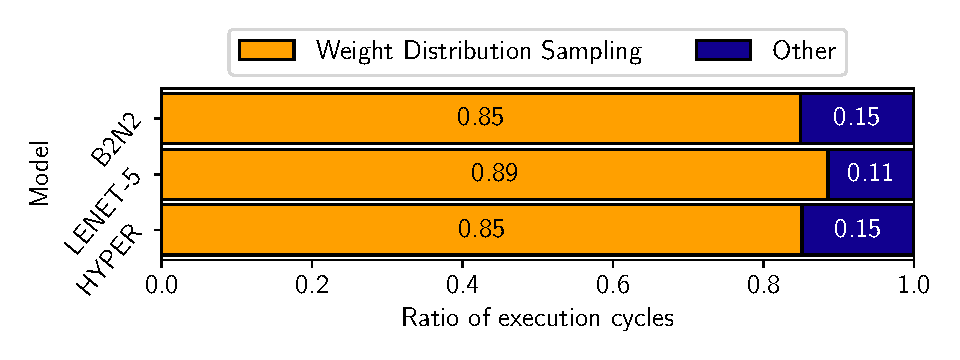
\includegraphics[width=0.9\textwidth]{root/Imagenes/bnn_lib/cycles.pdf}
	\caption{Ratio de ciclos de ejecución dedicados al muestreo de distribuciones gaussianas (amarillo) y al del resto de operaciones (azul) en las diferentes arquitecturas de modelos utilizadas.}
	\label{fig:cycle_profile}
\end{figure}

La operación de muestreo es la más costosa con diferencia, ocupando más del 80\% de los ciclos de ejecución en los 3 modelos diferentes. Por ello, uno de los objetivos principales de este trabajo y de otros relacionados ha sido optimizar esta operación.
